\section{Introduction}

Monitoring the state of the natural world is a key challenge of
ecological and biological research, since predicting future changes
depends on accurate observations of the present. Satellites give
observations at large scale but can only be applied to phenomena that
can be seen from far above, and are limited by cloud cover and other
atmospheric conditions.  Citizen science projects~\cite{citizensci,lostladybug} can
produce quality data, but require significant incentives to encourage
participation over large scale areas, and clever designs to derive
accurate data from untrained observers.  A potentially rich
alternative is to mine publicly-available social media for
observations relevant to natural world, in effect turning the billions
of social media users into citizen scientists without any explicit
actions on their part.  This idea is motivated by the large amount of
work that has  mined social media  to predict and
observe properties of the real world, including the stock
market~\cite{bollen11twitter},
elections~\cite{you2015multifacetedelections}, tourism
activity~\cite{wood2013usingtourism}, and so on.

However, most of this work has used textual data like Facebook posts
and Twitter feeds.  Social images are potentially a richer source of
information because they often include incidental evidence about the
natural world (Figure~\ref{fig:flickrexp}).  In addition, they record
visual documentation that can later be analyzed, inspected, and
validated; the danger of relying on text analysis and the importance
of validation was recently illustrated by the case of Google
Flu, which initially showed great promise in monitoring the spread of
influenza by mining search engine queries~\cite{ginsberg09flu}, but
was later found to be largely inaccurate~\cite{lazer2014parable}.
Of course, a key challenge in mining images is how to extract useful
semantic information.

\begin{figure}[t]
{\tiny{
\begin{center}
\begin{tabular}{@{}c@{\,\,\,}c@{\,\,\,}c@{\,\,\,}c@{\,\,\,}c@{\,\,\,}c@{\,\,\,}c@{\,\,\,}c@{\,\,\,}}
%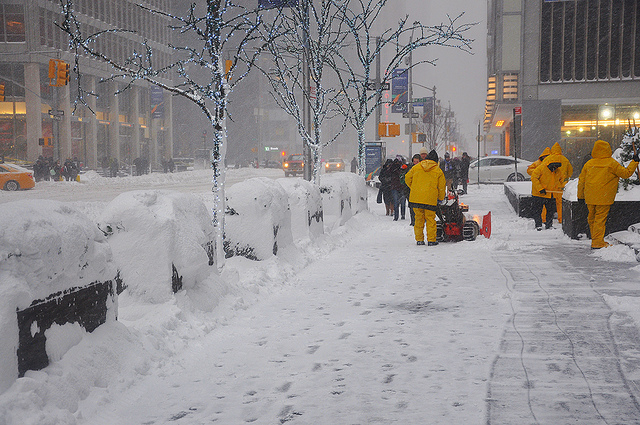
\includegraphics[width=0.12\textwidth]{image/citysnow.jpg} &
%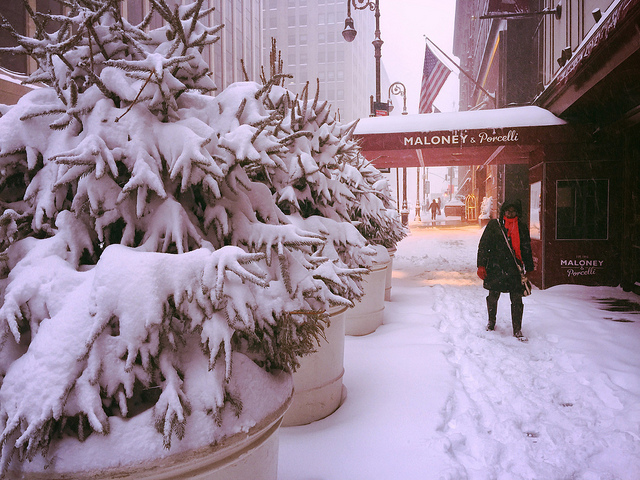
\includegraphics[width=0.1\textwidth]{image/citysnow2.jpg} &
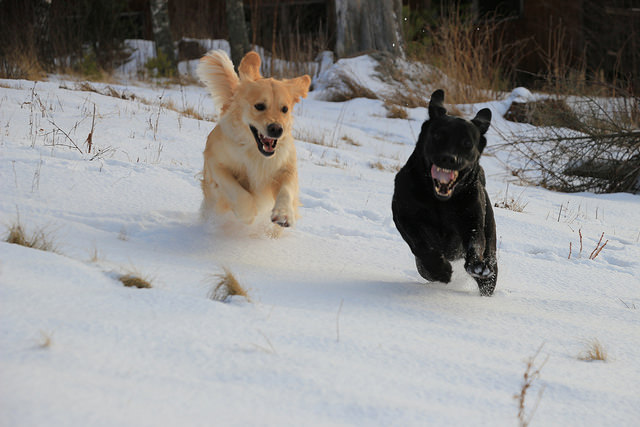
\includegraphics[width=0.15\textwidth,height=0.75in]{image/dogsnow.jpg} &
%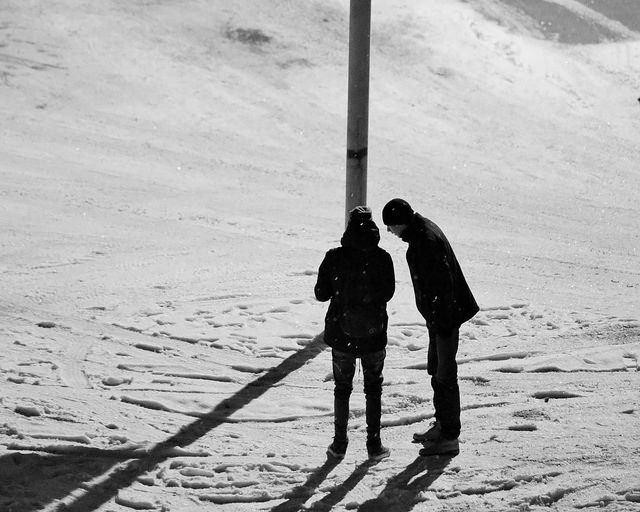
\includegraphics[width=0.1\textwidth]{image/humansnow.jpg} \\
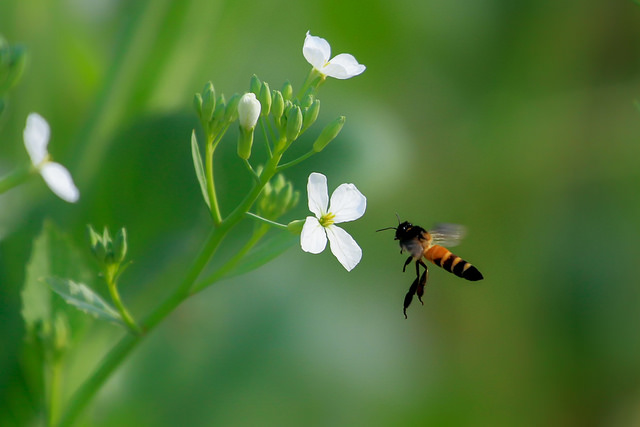
\includegraphics[width=0.15\textwidth,height=0.75in]{image/intentiongreen.jpg} &
%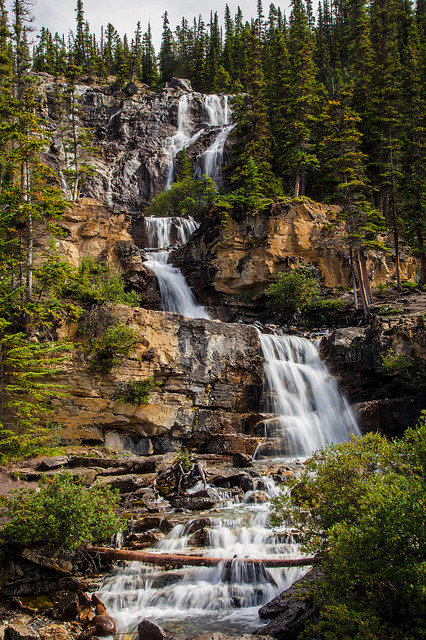
\includegraphics[width=0.1\textwidth]{image/waterfallgreen.jpg} &
%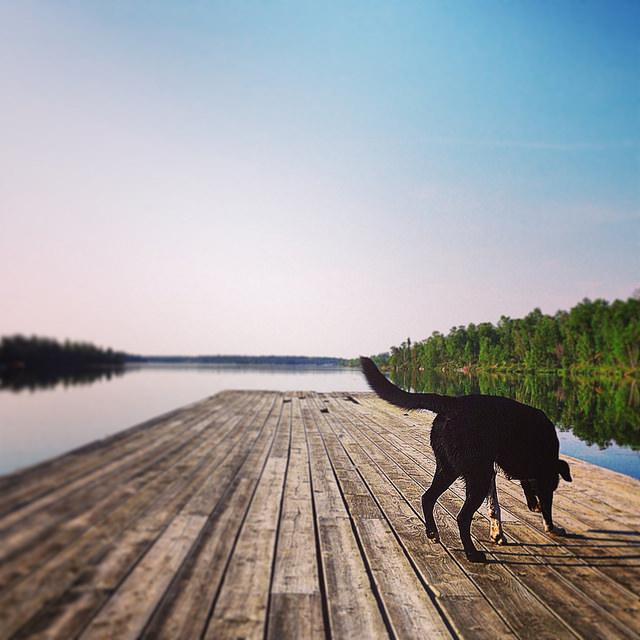
\includegraphics[width=0.12\textwidth,trim=0 0 0 cm,clip]{image/dogtree.jpg} &
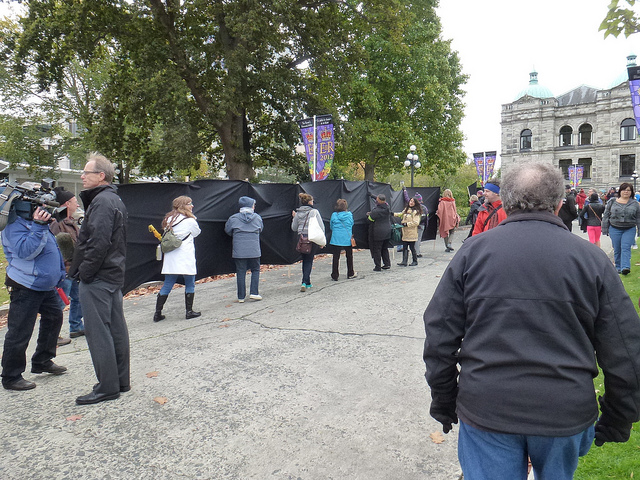
\includegraphics[width=0.15\textwidth,height=0.75in]{image/humantree.jpg} \\
\end{tabular}
\end{center}
}}
\vspace{-12pt}
\caption{Many social media images capture information about the state of the natural world, both intentionally or incidentally.}
\label{fig:flickrexp}
\vspace{-12pt}
\end{figure}


A few papers have begun to apply computer images for environmental
properties, including temperature~\cite{glasner2015hot}, cloud
cover~\cite{murdock2013webcam2satellite}, and smog conditions~\cite{li2015smog}. Most of
these papers use video data (e.g.\ from static webcams) so that visual
changes over time can be easily detected. Video camera feeds are
potentially very useful for studying longitudinal changes across time
in one particular place, but are limited to studying places where
cameras have been installed. Social photo sharing websites potentially
represent a complementary source of data, that give much greater
spatial coverage: whenever a user takes a photo at a particular place
and time and uploads it to Flickr, they are contributing a potentially
useful observation.

In this paper, we test the feasibility of leveraging these noisy and
biased images as a new source to observe nature, using modern deep
learning-based computer vision algorithms to recognize image content
automatically.  As a case study, we investigate two particular
phenomena, snowfall and vegetation coverage, since they are important
properties of the environment. They are relatively easy to recognize,
occur frequently in social images, and have satellite maps available
to serve as ground truth. This choice was also inspired by Fedorov et
al~\cite{fedorov2015snowwatch,fedorov2014snow}, who use video analysis
to monitor snow fall on mountains, and Zhang et
al~\cite{ecology2012www}, who predict snowfall from image collections
but using text tag analysis.  We first collect image data labeled to
reflect the presence or absence of ecology phenomena, and train
classifiers using Convolutional Neural Networks to recognize these
ecology phenomena in individual images. Of course, these classifiers
are noisy, and social image data is noisy also, with many inaccurate
timestamps and geo-tags.  We thus train an additional classifier that
examines all images taken at a given place and time, runs the image
classifier on each one, and then predicts if the phenomena actually
occured there and then.  Finally, we evaluate at a large scale,
training and testing on millions of Flickr images and quantiatively
evaluating the performance at hundreds of thousands of places and
times.

%% Inspried by an earlier work~\cite{ecology2012www} 
%% %\fxnote{ Fixed: cite{www}} 
%% analyzing ecology phenomenon from image tags only. We apply a new approach by 
%% understanding visual content of images, and run experiments on the exact same 
%% data set to study how vision techniques could help in social media data mining 
%% compared to using textual data alone. Also, to our best knowledge, among all the 
%% research works performing social sensing with image data, this is the first one 
%% providing continental scale quantitative performance evaluation.










\begin{figure}[t]
\centering
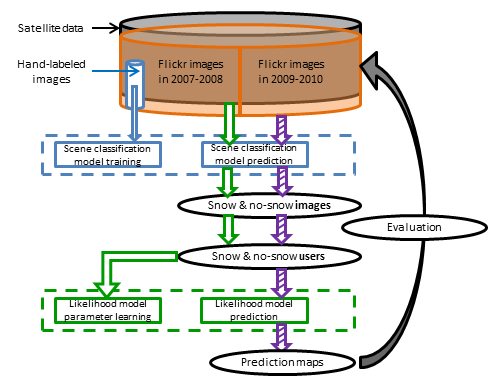
\includegraphics[scale=0.7]{figure/flowchartWevaluation.png}
\vspace{-12pt}
\caption{Overview of our approach. We train image classifiers(in blue) on large scale images. And by applying it to training images in 2007-2008, 
we train a likelihood model(in green) and finally make prediction by aggregating these visual evidence.}
% \fxnote{first classifier, then prediction}
\label{fig:overview}
\vspace{-12pt}
\end{figure}

